\chapter{Declarative Circuits}%
\label{ch:declarative}

Simplicity is a language for writing circuits:
A Simplicity program is a circuit.
%
In the following,
we give an account of the structure Simplicity and how it relates to traditional circuits.
In reality,
the Simplicity Bit Machine interprets a program in terms of types and executes it in terms of bits.
We ignore type theory for the moment and instead focus on how bits are modified by each operation.
By focusing on bits,
we can become more familiar with Simplicity without requiring extra theory.

\section{Traditional Circuits}

Circuits consist of \emph{gates},
which are their atomic building blocks,
connected via wires.
Traditionally,
these are \texttt{NOT}, \texttt{AND}, \texttt{OR}, etc.
Circuits compute \emph{Boolean functions},
i.e., functions that take a certain number of bits as input and produce a certain number of bits as output.
While gates already compute fundamental functions,
we can combine multiple gates to compute more complex functions.
An \texttt{XOR} and \texttt{AND} gate can be combined to form a half adder.
\texttt{XOR}, \texttt{AND} and \texttt{OR} form a full adder, etc.
Certain sets of gates can simulate other ones.
Gates \texttt{NOT} and \texttt{AND} can simulate all possible gates.
Alternatively,
gate \texttt{NAND} alone is also enough.
This enables us to write a circuit that computes \emph{any} Boolean function using only gates from the set.
We say,
the set of gates is \emph{functionally complete}.

\section{Simplicity Circuits}

Simplicity goes a slightly different route:
Wires carry a certain number of bits, like voltages,
and gates change the number of bits, like a change in voltage (down \emph{or up}).
Besides the number of bits,
each bit is either true of false \emph{(set or unset)}.
Each gate modifies the bitstring it receives based on the function that it computes.
%
To summarize,
wires in Simplicity circuits can carry multiple bits,
while traditional wires carry only one.
Simplicity circuits take a bitstring as input,
gates modify this bitstring
and the circuit produces a certain bitstring as a result.

In addition,
we work with gates that take a \emph{variable} number of input bits
and that produce a certain number of bits as result,
based on a mathematical function.
For instance,
a gate can take $n + m$ bits as input and produce $n$ bits as output.
Here,
the output function is $f(n, m) = n$.
Such a variable gate is called a gate \emph{schema}.
%
By assigning fixed values to variables,
we obtain a gate with a fixed number of inputs and outputs.
In the above example,
we could set $n \definedas 1$ and $m \definedas 2$
to obtain a gate that takes 3 bits of input to produce $1$ bit of output.
Such a fixed gate is called an \emph{instance} of the schema.

Schemata help us design circuits,
focusing on large mathematical functions that ultimately express spending conditions,
instead of focusing on tiny bits that do very little in the big picture.
When we evaluate a circuit on some input of fixed size,
then all variables are fixed and we end up with an instance.
This conversion from schema to instance happens in the background.
%
Simplicity circuits are \emph{declarative}:
Users define \emph{(declare)} the function they want to compute,
in terms of variables,
and the Bit Machine does the computation in the background.
Users never have to define how the evaluation is done,
just what they want to be evaluated.

\section{Combinators}%
\label{sec:combinators}

For convenience,
we make the wires in Simplicity circuits implicit by using \emph{combinators}:
A combinator takes zero to two circuits as argument and produces a larger circuit.
By recursively nesting combinators,
we can build larger and larger circuits.
%
This turns the circuit into a tree structure where combinators have up to two children.
There is a topmost combinator,
called the \emph{root}.
The bottommost combinators have no children and are called \emph{leaves}.
%
The root of each circuit determines its input and output type.
Bits are passed to the root as input,
the root passes these bits to its children,
the children return other bits as output,
and the root returns them as output.
This process of passing input through the children is repeated everywhere in the tree.

In the following,
the flow of bits will become obvious due to the wires.
We introduce each combinator,
illustrating the circuit that it represents
and explaining the function that it computes.
Boxes with variables $s, t$ stand for any circuit that is inserted into the diagram \emph{(a circuit variable)}.
The remaining boxes stand for gate schemata.
Each wire has a number that stands for its number of bits.
Bits always flow from left to right.

\subsection{Unit Constant}

\begin{center}
\begin{tikzpicture}
    \node (src) {};
    \node[gate, right=1cm of src] (0) {unit};
    \node[right=1cm of 0] (tgt) {};

    \draw (src) -- node[above]{$n$} (0);
    \draw (0) -- node[above]{$0$} (tgt);
\end{tikzpicture}
\end{center}

%
The unit combinator reads some number $n$ of bits and writes zero bits.
This is of little use on its own,
but serves as the foundation for bitstrings.
%
The number $n$ of read bits depends on the context,
i.e., how many bits are fed into \enquote{unit} via the surrounding circuit.
By default,
it holds that $n = 0$.

\subsection{Left Injection}

\begin{center}
\begin{tikzpicture}
    \node (src) {};
    \node[subcircuit, right=1cm of src] (0) {$t$};
    \node[gate, right=1cm of 0] (1) {injl};
    \node[right=3cm of 1] (tgt) {};

    \draw (src) -- node[above]{$n$} (0);
    \draw (0) -- node[above]{$m$} (1);
    \draw (1) -- node[above]{$1 + \max(m,o)$} (tgt);
\end{tikzpicture}
\end{center}

%
The left injection combinator takes one argument---%
circuit $t$ that reads $n$ bits and writes $m$ bits---%
and places its output in a \emph{union} as \emph{left} value.
%
Length $o$ of the \emph{right} type depends on the context,
i.e., how many bits are read from \enquote{injl} via the surrounding circuit.
By default, it holds that $o = 0$.
%
A \emph{(tagged) union} is a type that can contain values from a fixed set of types,
but only one at a time.
Which type is contained is encoded in the \emph{tag} which is part of the union.
In Simplicity,
unions have a \emph{left} type and a \emph{right} type.
The tag is therefore a simple bit,
which is \enquote{false} if a left value is contained and \enquote{true} if a right value is contained.
Given a left type of length $m$ and a right type of length $o$,
the length of their union is $1 + \max(m, o)$.
\emph{This helps with memory alignment. The shorter type is padded internally.}

\subsection{Right Injection}

\begin{center}
\begin{tikzpicture}
    \node (src) {};
    \node[subcircuit, right=1cm of src] (0) {$t$};
    \node[gate, right=1cm of 0] (1) {injr};
    \node[right=3cm of 1] (tgt) {};

    \draw (src) -- node[above]{$n$} (0);
    \draw (0) -- node[above]{$o$} (1);
    \draw (1) -- node[above]{$1 + \max(m,o)$} (tgt);
\end{tikzpicture}
\end{center}

%
The right injection combinator takes one argument---%
circuit $t$ that reads $n$ bits and writes $o$ bits---%
and places its output in a \emph{union} as \emph{right} value.
Again,
length $m$ of the left type depends on the context
and it is zero by default.
%
With injections, we can produce bits:
By wrapping $m$ bits in a union as left value via \enquote{injl},
we add a \enquote{false} bit at the front.
By wrapping $o$ bits in a union as right value via \enquote{injr},
we add a \enquote{true} bit.
If circuit $t$ is \enquote{unit},
then we obtain a circuit that produces a constant \enquote{false} or \enquote{true} no matter the input.

\subsection{Pair}

\begin{center}
\begin{tikzpicture}
    \node (src) {};
    \node[crossing, right=1cm of src] (0) {};
    \node[subcircuit, above right=0.25cm and 0.5cm of 0] (00) {$s$};
    \node[subcircuit, below right=0.25cm and 0.5cm of 0] (01) {$t$};
    \node[pair, right=1.25cm of 0] (1) {$+$};
    \node[right=1cm of 1] (tgt) {};

    \draw (src) -- node[above]{$n$} (0);
    \draw (0) |- (00);
    \draw (0) |- (01);
    \draw (1) |- node[above]{$m$} (00);
    \draw (1) |- node[below]{$o$} (01);
    \draw (1) -- node[above]{$m+o$} (tgt);
\end{tikzpicture}
\end{center}

%
The pair combinator takes two arguments---%
circuit $s$ that reads $n$ bits and writes $m$ bits,
and circuit $t$ that reads $n$ bits and writes $o$ bits---%
and \emph{concatenates} their outputs.
That is,
the overall input becomes the input of both circuits,
and the overall output is the output of the first circuit followed by the output of the second circuit.
%
With concatenation,
we can produce arbitrary bitstrings:
Simply concatenate as many bits, produced by injections, as necessary.
%
By nesting the unit, injection and pair combinators,
we can write a circuit that produces any bitstring as constant output.

\subsection{Take}

\begin{center}
\begin{tikzpicture}
    \node (src) {};
    \node[gate, right=1.5cm of src] (0) {take};
    \node[subcircuit, right=1cm of 0] (1) {$t$};
    \node[right=1cm of 1] (tgt) {};

    \draw (src) -- node[above]{$n+m$} (0);
    \draw (0) -- node[above]{$n$} (1);
    \draw (1) -- node[above]{$o$} (tgt);
\end{tikzpicture}
\end{center}

%
The take combinator takes one argument---%
circuit $t$ that reads $n$ bits and writes $o$ bits---%
and evaluates it on the \emph{first $n$ bits} of the overall input.
That is,
the first $n$ bits the input are \emph{taken} and the remaining $m$ bits are discarded.
The number $m$ depends on the context,
i.e., how many bits are fed into \enquote{take} via the surrounding circuit.
By default, it holds that $m = 0$.

\subsection{Drop}

\begin{center}
\begin{tikzpicture}
    \node (src) {};
    \node[gate, right=1.5cm of src] (0) {drop};
    \node[subcircuit, right=1cm of 0] (1) {$t$};
    \node[right=1cm of 1] (tgt) {};

    \draw (src) -- node[above]{$n+m$} (0);
    \draw (0) -- node[above]{$m$} (1);
    \draw (1) -- node[above]{$o$} (tgt);
\end{tikzpicture}
\end{center}

%
The drop combinator takes on argument---%
circuit $t$ that reads $m$ bits and writes $o$ bits---%
and evaluates it on the \emph{last $m$ bits} of the overall input.
That is,
the first $n$ bits of the input are \emph{dropped} and the remaining $m$ bits are used as input for $t$.
Again,
number $n$ depends on the context and it is zero by default.
%
By recursively nesting the take and drop combinators,
we can deconstruct bitstrings in arbitrary ways:
We can write circuits that take a bitstring of given length as input and return any sub-slice of it.

\subsection{Identity}

\begin{center}
\begin{tikzpicture}
    \node (src) {};
    \node[gate, right=1cm of src] (0) {iden};
    \node[right=1cm of 0] (tgt) {};

    \draw (src) -- node[above]{$n$} (0);
    \draw (0) -- node[above]{$n$} (tgt);
\end{tikzpicture}
\end{center}

%
The identity combinator reads $n$ bits and writes the same $n$ bits.
The circuit therefore computes the \emph{identity} function.
%
It is often used in conjunction with \enquote{take} and \enquote{drop}
to produce a subslice of a given bitstring,
or to keep a copy of the input in one branch of a pair while the other branch computes something.
There is no other circuit that passes through the input.

\subsection{Composition}

\begin{center}
\begin{tikzpicture}
    \node (src) {};
    \node[subcircuit, right=1cm of src] (0) {$s$};
    \node[subcircuit, right=1cm of 0] (1) {$t$};
    \node[right=1cm of 1] (tgt) {};

    \draw (src) -- node[above]{$n$} (0);
    \draw (0) -- node[above]{$m$} (1);
    \draw (1) -- node[above]{$o$} (tgt);
\end{tikzpicture}
\end{center}

%
The composition combinator takes two arguments---%
circuit $s$ that reads $n$ bits and writes $m$ bits,
and circuit $t$ that reads $m$ bits and writes $o$ bits---%
and \emph{composes} the two circuits.
That is,
the overall input becomes the input of the first circuit,
whose output becomes the input of the second circuit,
whose output becomes the overall output.
%
In programming, this is also called \emph{chaining} or \emph{piping}.

\subsection{Case}

\begin{center}
\begin{tikzpicture}
    \node (src) {};
    \node[gate, right=3.5cm of src] (0) {case};
    \node[subcircuit, above right=0.25cm and 0.25cm of 0] (1) {$s$};
    \node[subcircuit, below right=0.25cm and 0.25cm of 0] (2) {$t$};
    \node[crossing, right=1.25cm of 0] (3) {};
    \node[right=1cm of 3] (tgt) {};

    \draw (src) -- node[above]{$1+\max(n,m)+o$} (0);
    \draw (0) |- node[above]{$n+o$} (1);
    \draw (0) |- node[below]{$m+o$} (2);
    \draw (3) |- (1);
    \draw (3) |- (2);
    \draw (3) -- node[above]{$p$} (tgt);
\end{tikzpicture}
\end{center}

%
The case combinator takes two arguments---%
circuit $s$ that reads $n + o$ bits and writes $o$ bits,
and circuit $t$ that reads $m + o$ bits and writes $o$ bits---%
and \emph{branches} to either circuit depending on its input.
The input consists of a union of a left type of length $n$ and a right type of length $m$,
concatenated with $o$ additional bits.
If the tag is zero,
then the union contains a left value and circuit $s$ is evaluated on the left value plus the trailing $o$ bits.
If the tag is one,
then circuit $t$ is evaluated on the contained right value plus the trailing bits.
Note how the first bits of the input of $s$ and $t$ differ,
while the remaining input and output are the same.
%
In programming,
the case combinator corresponds to an \emph{if-statement}.
Given the (de)construction of arbitrary bitstrings and the three functional primitives above,
we can compute any Boolean function using some circuit.

%\section{Term notation}
%
% writing Simplicity programs as terms

\section{Examples}%
\label{sec:examples}

Let us look at some examples of Simplicity programs that compute useful functions.
As already said,
Simplicity is functionally complete,
i.e.,
for each Boolean function there is a program that computes said function.
Any decidable spending condition can be expressed in a program that might or might not be small.
If the program ends up large,
its size can be reduced by using so-called \emph{jets} (see Section~\ref{sec:jets}).

Note:
We deliberately keep algebraic expressions $x+y$, $\max(x,y)$ and the parentheses as they are,
even though it might seem natural to resolve them.
It is important to keep them separate,
because the combinators will break them down again.

\subsection{False Constant}

\begin{center}
\begin{tikzpicture}
    \node (src) {};
    \node[gate, right=1cm of src] (0) {unit};
    \node[gate, right=1cm of 0] (1) {injl};
    \node[right=3cm of 1] (tgt) {};

    \draw (src) -- node[above]{$n$} (0);
    \draw (0) -- node[above]{$0$} (1);
    \draw (1) -- node[above]{$1 + \max(0,0)$} (tgt);
\end{tikzpicture}
\begin{tikzpicture}
    \node (src) {};
    \node[gate, right=1cm of src] (0) {false};
    \node[right=1cm of 0] (tgt) {};

    \draw (src) -- node[above]{$n$} (0);
    \draw (0) -- node[above]{$1$} (tgt);
\end{tikzpicture}
\end{center}

%
By nesting the unit constant in a left injection,
we obtain a circuit that produces a constant \enquote{false} bit no matter the input \emph{(see left)}.
The $n$ input bits are variable and depend on the surrounding circuit.
The input is passed to \enquote{unit},
which passes $0$ bits to \enquote{injl},
which in turn wraps these $0$ bits in a union as left value.
The length of the right value of this union is also $0$ bits,
so the length of the union is $1$ bit,
which is what we wanted.
%
As a shorthand,
we can write the \enquote{false} circuit as a gate \emph{(see right)}.

\subsection{True Constant}

\begin{center}
\begin{tikzpicture}
    \node (src) {};
    \node[gate, right=1cm of src] (0) {unit};
    \node[gate, right=1cm of 0] (1) {injr};
    \node[right=3cm of 1] (tgt) {};

    \draw (src) -- node[above]{$n$} (0);
    \draw (0) -- node[above]{$0$} (1);
    \draw (1) -- node[above]{$1 + \max(0,0)$} (tgt);
\end{tikzpicture}
\begin{tikzpicture}
    \node (src) {};
    \node[gate, right=1cm of src] (0) {true};
    \node[right=1cm of 0] (tgt) {};

    \draw (src) -- node[above]{$n$} (0);
    \draw (0) -- node[above]{$1$} (tgt);
\end{tikzpicture}
\end{center}

%
By nesting the unit constant in a right injection,
we obtain a circuit that produces a constant \enquote{true} bit no matter the input \emph{(see left)}.
The computation is analogous to that of the false constant.
As a shorthand,
wer can write the \enquote{true} circuit as a gate \emph{(see right)}.

\subsection{Condition}

\begin{center}
\begin{tikzpicture}
    \node (src) {};
    \node[gate, right=3.5cm of src] (0) {case};
   
    % top branch
    \node[gate, above right=0.25cm and 0.25cm of 0] (10) {drop};
    \node[subcircuit, right=1cm of 10] (11) {$t$};
    \draw (10) -- node[above]{$n$} (11);
    \node[subcircuit, fit=(10) (11)] (1) {};

    % bottom branch
    \node[gate, below right=0.25cm and 0.25cm of 0] (20) {drop};
    \node[subcircuit, right=1cm of 20] (21) {$s$};
    \draw (20) -- node[above]{$n$} (21);
    \node[subcircuit, fit=(20) (21)] (2) {};

    \node[crossing, right=3.25cm of 0] (3) {};
    \node[right=1cm of 3] (tgt) {};

    \draw (src) -- node[above]{$1+\max(0,0)+n$} (0);
    \draw (0) |- node[above]{$0+n$} (10);
    \draw (0) |- node[below]{$0+n$} (20);
    \draw (3) |- (11);
    \draw (3) |- (21);
    \draw (3) -- node[above]{$m$} (tgt);
\end{tikzpicture}
\begin{tikzpicture}
    \node (src) {};
    \node[gate, right=1.5cm of src] (0) {cond};
    \node[subcircuit, above right=0.25cm and 0.25cm of 0] (1) {$t$};
    \node[subcircuit, below right=0.25cm and 0.25cm of 0] (2) {$s$};
    \node[crossing, right=1.25cm of 0] (3) {};
    \node[right=1cm of 3] (tgt) {};

    \draw (src) -- node[above]{$1+n$} (0);
    \draw (0) |- node[above]{$n$} (1);
    \draw (0) |- node[below]{$n$} (2);
    \draw (3) |- (1);
    \draw (3) |- (2);
    \draw (3) -- node[above]{$m$} (tgt);
\end{tikzpicture}
\end{center}

%
By nesting drop circuits in a case circuit,
we obtain a circuit that resembles an \enquote{if-else-statement} \emph{(see left)}:
The circuit takes two arguments---%
circuits $s$ and $t$ that read $n$ bits and write $m$ bits,
respectively---%
and branches to either of them based on the tag bit of the input.
Circuit $s$ corresponds to the \enquote{if} clause
and circuit $t$ to the \enquote{else} clause.
\emph{To avoid confusion,
we consistently put negative branches above positive ones,
like for \enquote{case},
so the order of $s$ and $t$ is reversed.}
If the tag bit is false,
then $0 + n$ bits are passed to the top \enquote{drop},
which passes $n$ bits to $t$,
which in turn produces $m$ output bits.
If the tag bit is true,
then the bottom branch produces $m$ output bits.
%
As a shorthand,
we can write the \enquote{cond} circuit as a gate \emph{(see right)}.

\subsection{Negation}

\begin{center}
\begin{tikzpicture}
    \node (src) {};

    % pair (t unit) -- cond true false
    % pair (t unit)
    \node[crossing, right=1cm of src] (0) {};
    \node[subcircuit, above right=0.25cm and 0.5cm of 0] (00) {$t$};
    \node[gate, below right=0.25cm and 0.5cm of 0] (01) {unit};
    \node[pair, right=1.75cm of 0] (1) {$+$};

    \draw (0) |- (00);
    \draw (0) |- (01);
    \draw (1) |- node[above] (label1a) {$1$} (00);
    \draw (1) |- node[below] (label1b) {$0$} (01);
    \node[subcircuit, fit=(0) (00) (01) (1) (label1a) (label1b)] (0-1) {};
    % end pair

    % cond true false
    \node[gate, right=1.5cm of 1] (2) {cond};
    \node[gate, above right=0.25cm and 0.25cm of 2] (20) {true};
    \node[gate, below right=0.25cm and 0.25cm of 2] (21) {false};
    \node[crossing, right=1.75cm of 2] (3) {};

    \draw (1)  -- node[above]{$1+0$} (2);
    \draw (2) |- node[above] (label20) {$0$} (20);
    \draw (2) |- node[below] (label21) {$0$} (21);
    \draw (3) |- (20);
    \draw (3) |- (21);
    \node[subcircuit, fit=(2) (20) (21) (3) (label20) (label21)] (2-3) {};
    % end cond

    \node[right=1cm of 3] (tgt) {};

    \draw (src) -- node[above]{$n$} (0);
    \draw (3)  -- node[above]{$1$} (tgt);
\end{tikzpicture}
\begin{tikzpicture}
    \node (src) {};
    \node[subcircuit, right=1cm of src] (0) {$t$};
    \node[gate, right=1cm of 0] (1) {not};
    \node[right=1cm of 1] (tgt) {};

    \draw (src) -- node[above]{$n$} (0);
    \draw (0) -- node[above]{$1$} (1);
    \draw (1) -- node[above]{$1$} (tgt);
\end{tikzpicture}
\end{center}

%
Now we show how traditional gates are represented as Simplicity circuits:
The negation circuit takes one argument---%
circuit $t$ that reads $n$ bits and writes $1$ bit---%
and negates this output \emph{(see left)}.
First,
a pair joins the output of $t$ with zero bits.
Second,
a condition evaluates the first bit
and passes the remaining zero bits to either top or bottom branch.
If the first bit is false,
then the top branch produces a constant \enquote{true}.
Otherwise,
the bottom branch produces \enquote{false}.
The zero bits are ignored.
As you can see,
the output is \enquote{true} if $t$ produces \enquote{false} and vice versa.
%
As a shorthand,
we can write the \enquote{not} circuit as a gate \emph{(see right)}.

\subsection{Conjunction}

\begin{center}
\begin{tikzpicture}
    \node (src) {};

    % pair (s iden) -- cond false t
    % pair (s iden)
    \node[crossing, right=1cm of src] (0) {};
    \node[subcircuit, above right=0.25cm and 0.5cm of 0] (00) {$s$};
    \node[gate, below right=0.25cm and 0.5cm of 0] (01) {iden};
    \node[pair, right=1.75cm of 0] (1) {$+$};

    \draw (0) |- (00);
    \draw (0) |- (01);
    \draw (1) |- node[above] (label1a) {$1$} (00);
    \draw (1) |- node[below] (label1b) {$n$} (01);
    \node[subcircuit, fit=(0) (00) (01) (1) (label1a) (label1b)] (0-1) {};
    % end pair

    % cond false t
    \node[gate, right=1.5cm of 1] (2) {cond};
    \node[gate, above right=0.25cm and 0.25cm of 2] (20) {false};
    \node[subcircuit, below right=0.25cm and 0.25cm of 2] (21) {$t$};
    \node[crossing, right=1.75cm of 2] (3) {};

    \draw (1)  -- node[above]{$1+n$} (2);
    \draw (2) |- node[above] (label20) {$n$} (20);
    \draw (2) |- node[below] (label21) {$n$} (21);
    \draw (3) |- (20);
    \draw (3) |- (21);
    \node[subcircuit, fit=(2) (20) (21) (3) (label20) (label21)] (2-3) {};
    % end cond

    \node[right=1cm of 3] (tgt) {};

    \draw (src) -- node[above]{$n$} (0);
    \draw (3)  -- node[above]{$1$} (tgt);
\end{tikzpicture}
\begin{tikzpicture}
    \node (src) {};
    \node[crossing, right=1cm of src] (0) {};
    \node[subcircuit, above right=0.25cm and 0.5cm of 0] (00) {$s$};
    \node[subcircuit, below right=0.25cm and 0.5cm of 0] (01) {$t$};
    \node[gate, right=1.25cm of 0] (1) {and};
    \node[right=1cm of 1] (tgt) {};

    \draw (src) -- node[above]{$n$} (0);
    \draw (0) |- (00);
    \draw (0) |- (01);
    \draw (1) |- node[above]{$1$} (00);
    \draw (1) |- node[below]{$1$} (01);
    \draw (1) -- node[above]{$1$} (tgt);
\end{tikzpicture}
\end{center}

%
The conjunction circuit takes two arguments---%
circuits $s$ and $t$ that read $n$ bits and write $1$ bit, respectively---%
and computes the logical conjunction of both outputs \emph{(see left)}.
First,
a pair joins the output of $s$ with a copy of the original $n$ input bits.
Second,
a condition evaluates the first bit
and passes the remaining $n$ bits to either top or bottom branch.
If the first bit is false,
then the top branch produces a constant \enquote{false}.
Otherwise,
the bottom branch evaluates $t$ on the $n$ input bits.
As you can see,
the output is \enquote{true} if both $s$ and $t$ produce \enquote{true}
and \enquote{false} otherwise.
%
As a shorthand,
we can write the \enquote{and} circuit as a gate \emph{(see right)}.

\subsection{Disjunction}

\begin{center}
\begin{tikzpicture}
    \node (src) {};

    % pair (s iden) -- cond t true
    % pair (s iden)
    \node[crossing, right=1cm of src] (0) {};
    \node[subcircuit, above right=0.25cm and 0.5cm of 0] (00) {$s$};
    \node[gate, below right=0.25cm and 0.5cm of 0] (01) {iden};
    \node[pair, right=1.75cm of 0] (1) {$+$};

    \draw (0) |- (00);
    \draw (0) |- (01);
    \draw (1) |- node[above] (label1a) {$1$} (00);
    \draw (1) |- node[below] (label1b) {$n$} (01);
    \node[subcircuit, fit=(0) (00) (01) (1) (label1a) (label1b)] (0-1) {};
    % end pair

    % cond t true
    \node[gate, right=1.5cm of 1] (2) {cond};
    \node[subcircuit, above right=0.25cm and 0.25cm of 2] (20) {$t$};
    \node[gate, below right=0.25cm and 0.25cm of 2] (21) {true};
    \node[crossing, right=1.75cm of 2] (3) {};

    \draw (1)  -- node[above]{$1+n$} (2);
    \draw (2) |- node[above] (label20) {$n$} (20);
    \draw (2) |- node[below] (label21) {$n$} (21);
    \draw (3) |- (20);
    \draw (3) |- (21);
    \node[subcircuit, fit=(2) (20) (21) (3) (label20) (label21)] (2-3) {};
    % end cond

    \node[right=1cm of 3] (tgt) {};

    \draw (src) -- node[above]{$n$} (0);
    \draw (3)  -- node[above]{$1$} (tgt);
\end{tikzpicture}
\begin{tikzpicture}
    \node (src) {};
    \node[crossing, right=1cm of src] (0) {};
    \node[subcircuit, above right=0.25cm and 0.5cm of 0] (00) {$s$};
    \node[subcircuit, below right=0.25cm and 0.5cm of 0] (01) {$t$};
    \node[gate, right=1.25cm of 0] (1) {or};
    \node[right=1cm of 1] (tgt) {};

    \draw (src) -- node[above]{$n$} (0);
    \draw (0) |- (00);
    \draw (0) |- (01);
    \draw (1) |- node[above]{$1$} (00);
    \draw (1) |- node[below]{$1$} (01);
    \draw (1) -- node[above]{$1$} (tgt);
\end{tikzpicture}
\end{center}

%
The disjunction circuit takes two arguments---%
circuits $s$ and $t$ that read $n$ bits and write $1$ bit, respectively---%
and computes the logical disjunction of both outputs \emph{(see left)}.
The pair-condition construction is just as for conjunction,
but with different branches:
If the first bit (from $s$) is false,
then the top branch evaluates $t$ on the $n$ input bits.
Otherwise,
the bottom branch produces a constant \enquote{true}.
As you can see,
the output is \enquote{false} if both $s$ and $t$ produce \enquote{false}
and \enquote{true} otherwise.
%
As a shorthand,
we can write the \enquote{or} circuit as a gate \emph{(see right)}.

\subsection{Half Adder}

\begin{center}
\begin{tikzpicture}
    \node (src) {};
    \node[gate, right=1.5cm of src] (0) {cond};
   
    % top branch
    %% pair
    \node[crossing, above right=1.25cm and 0.25cm of 0] (10) {};
    \node[gate, above right=0.25cm and 0.5cm of 10] (11) {false};
    \node[gate, below right=0.25cm and 0.5cm of 10] (12) {iden};
    \node[pair, right=1.75cm of 10] (13) {$+$};

    \draw (10) |- (11);
    \draw (10) |- (12);
    \draw (13) |- node[above] (label11) {$1$} (11);
    \draw (13) |- node[below] (label12) {$1$} (12);
    \node[subcircuit, fit=(10) (11) (12) (13) (label11) (label12)] (1) {};
    %% end pair

    % bottom branch
    %% pair
    \node[crossing, below right=1.25cm and 0.25cm of 0] (20) {};
    \node[gate, above right=0.5cm and 0.5cm of 20] (21) {iden};

    %%% not
    \node[gate, below right=0.5cm and 0.5cm of 20] (220) {iden};
    \node[gate, right=1cm of 220] (221) {not};

    \draw (220) -- node[above] (label220) {$1$} (221);
    \node[subcircuit, fit=(220) (221) (label220)] (22) {};
    %%% end not

    \node[pair, right=3.75cm of 20] (23) {$+$};

    \draw (20) |- (21);
    \draw (20) |- (220);
    \draw (23) |- node[above] (label21) {$1$} (21);
    \draw (23) |- node[below] (label22) {$1$} (221);
    \node[subcircuit, fit=(20) (21) (22) (23) (label21) (label22)] (1) {};
    %% end pair

    \node[crossing, right=5cm of 0] (3) {};
    \node[right=1.5cm of 3] (tgt) {};

    \draw (src) -- node[above]{$1+1$} (0);
    \draw (0) |- node[above]{$1$} (10);
    \draw (0) |- node[below]{$1$} (20);
    \draw (3) |- (13);
    \draw (3) |- (23);
    \draw (3) -- node[above]{$1+1$} (tgt);
\end{tikzpicture}
\end{center}

%
We can combine the above gates to construct arithmetic circuits of any kind,
like adders, subtractors and multipliers.
For brevity sake,
we limit ourselves to a very simple circuit, namely the half adder:
The circuit reads 2 bits $a$ and $b$, adds them and writes 2 output bits $c$ and $s$ as a result.
The first output $c$ is the carry bit while the second output $s$ is the sum modulo two.
%
If $a$ is \enquote{false},
then the top branch receives $b$.
A pair joins a constant \enquote{false} with $b$ and passes that to the output.
That is,
the carry bit is always false and the sum bit equals $b$.
This makes sense,
since $0 + b = b$ carry 0.
%
If $a$ is \enquote{true},
then the bottom branch receives $b$.
A pair joins a copy of $b$ with the negation of $b$ and passes that to the output.
That is,
the carry bit equals $b$ and the sum is the negation of $b$.
This makes sense,
since $1 + 0 = 1$ carry 0
and $1 + 1 = 0$ carry 1.

\subsection{Scribe}%
\label{ssec:scribe}

\begin{center}
\begin{minipage}{0.5\textwidth}
\begin{tikzpicture}
    \node (src) {};
    \node[gate, right=1cm of src] (0) {unit};
    \node[right=1cm of 0] (tgt) {};

    \draw (src) -- node[above]{$n$} (0);
    \draw (0) -- node[above]{$0$} (tgt);
\end{tikzpicture}

\begin{tikzpicture}
    \node (src) {};
    \node[subcircuit, right=1cm of src] (0) {$\text{scribe}(b)$};
    \node[gate, right=1cm of 0] (1) {injl};
    \node[right=3cm of 1] (tgt) {};

    \draw (src) -- node[above]{$n$} (0);
    \draw (0) -- node[above]{$|b|$} (1);
    \draw (1) -- node[above]{$1 + \max(|b|,o)$} (tgt);
\end{tikzpicture}

\begin{tikzpicture}
    \node (src) {};
    \node[subcircuit, right=1cm of src] (0) {$\text{scribe}(b)$};
    \node[gate, right=1cm of 0] (1) {injr};
    \node[right=3cm of 1] (tgt) {};

    \draw (src) -- node[above]{$n$} (0);
    \draw (0) -- node[above]{$|b|$} (1);
    \draw (1) -- node[above]{$1 + \max(m,|b|)$} (tgt);
\end{tikzpicture}
\end{minipage}
%\hspace{0cm}
\begin{minipage}{0.3\textwidth}
\begin{tikzpicture}
    \node (src) {};
    \node[crossing, right=1cm of src] (0) {};
    \node[subcircuit, above right=0.25cm and 0.5cm of 0] (00) {$\text{scribe}(b)$};
    \node[subcircuit, below right=0.25cm and 0.5cm of 0] (01) {$\text{scribe}(c)$};
    \node[pair, right=2.75cm of 0] (1) {$+$};
    \node[right=1cm of 1] (tgt) {};

    \draw (src) -- node[above]{$n$} (0);
    \draw (0) |- (00);
    \draw (0) |- (01);
    \draw (1) |- node[above]{$|b|$} (00);
    \draw (1) |- node[below]{$|b|$} (01);
    \draw (1) -- node[above]{$|bc|$} (tgt);
\end{tikzpicture}
\end{minipage}
\end{center}

%
Simplicity's functional completeness includes one special case,
namely the ability to produce any constant in a circuit no matter the input.
For each bitstring $a$ that we want to produce,
there exists such a circuit which we call $\text{scribe}(a)$.
%
If $a$ is the empty string,
then $\text{scribe}(a)$ is the unit constant \emph{(see top left)}.
%
If $a$ is a \enquote{false} bit followed by bitstring $b$,
then we can produce it by passing the output of $\text{scribe}(b)$,
which produces $b$,
into a left injection \emph{(see middle left)}.
This adds a false tag bit in front of $b$.
Note that in principle,
the length $o$ of the right type of this union could be nonzero,
but for our purposes we may assume it to be zero.
%
If $a$ is a \enquote{true} bit followed by bitstring $b$,
then we pass the output of $\text{scribe}(y)$ into a right injection,
analogous to the above \emph{(see bottom left)}.
Again,
we assume the length $m$ to be zero.
%
If $a$ is the concatenation of two bitstrings $b$ and $c$,
then we join the outputs of $\text{scribe}(b)$ and $\text{scribe}(c)$ in a pair \emph{(see right)}.
%
In all cases,
the input is completely ignored and a constant output is produced.

\section{Merkle Roots}%
\label{sec:merkle}

Programs have a tree structure:
The outermost combinator, called \emph{root},
forms the entire circuit and determines the program's input and output type.
Other combinators are recursively nested in the root as arguments,
according to the respective combinator's definition (see Section~\ref{sec:combinators}).
At the bottom of this tree are combinators without arguments,
called \emph{leaves}.

\begin{center}
\begin{tikzpicture}
    \node (src) {};

    % pair (pair _ _) _ -- _
    % pair (pair _ _) _
    \node[crossing, right=1cm of src] (0) {};
   
    %% pair _ _
    \node[crossing, above right=1cm and 0.5cm of 0] (00) {};
    \node[gate, above right=0.25cm and 0.5cm of 00] (000) {\phantom{unit}};
    \node[gate, below right=0.25cm and 0.5cm of 00] (001) {\phantom{unit}};
    \node[pair, right=1.75cm of 00] (01) {$+$};

    \draw (00) |- (000);
    \draw (00) |- (001);
    \draw (01) |- (000);
    \draw (01) |- (001);
    \node[above right=-0.1cm and -0.1cm of 000] (label000) {$M_0$};
    \node[below right=-0.1cm and -0.1cm of 001] (label001) {$M_1$};
    \node[subcircuit, fit=(00) (000) (001) (01) (label000) (label001)] (00-01) {};
    \node[above right=-0.1cm and -0.1cm of 00-01] (label00-01) {$M_2$};
    %% end pair

    %% _
    \node[gate, below right=1cm and 0.5cm of 0] (02) {\phantom{unit}};
    \node[above right=-0.1cm and -0.1cm of 02] (label02) {$M_3$};
    %% end

    \node[pair, right=3cm of 0] (1) {$+$};

    \draw (0) |- (00);
    \draw (0) |- (02);
    \draw (1) |- (01);
    \draw (1) |- (02);
    \node[subcircuit, fit=(0) (00-01) (02) (1) (label00-01) (label02)] (0-1) {};
    \node[above right=-0.1cm and -0.1cm of 0-1] (label0-1) {$M_4$};
    % end pair

    % _
    \node[gate, right=1cm of 1] (2) {\phantom{unit}};
    \node[above right=-0.1cm and -0.1cm of 2] (label2) {$M_5$};

    \draw (1) -- (2);
    % end _

    \node[right=1cm of 2] (tgt) {};

    \draw (src) -- (0);
    \draw (2) -- (tgt);
    \node[subcircuit, fit=(src) (0-1) (2) (tgt) (label0-1) (label2)] (src-tgt) {};
    \node[above right=-0.1cm and -0.1cm of src-tgt] (labelsrc-tgt) {$M_6$};
\end{tikzpicture}
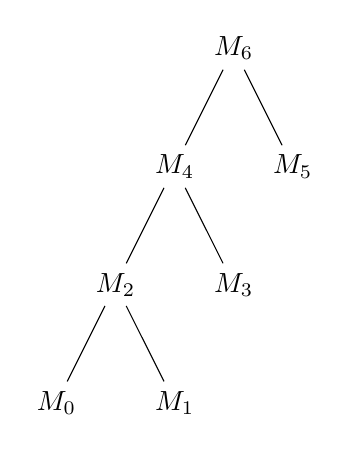
\begin{tikzpicture}
    \node {$M_6$}
        child { node {$M_4$}
            child { node {$M_2$}
                child { node {$M_0$} }
                child { node {$M_1$} }
            }
            child { node {$M_3$} }
        }
        child { node {$M_5$} };
\end{tikzpicture}
\end{center}

%
Above is an illustration of a circuit with its nested combinators (dashed boxes).
Each combinator has a Merkle root which uniquely identifies it and which is computed from its arguments.
On the right is an illustration of the corresponding tree structure of the circuit.

\subsection{Commitment Merkle Root}

The commitment Merkle root (CMR) uniquely identifies a program at \emph{commitment time}.
At this time,
we define a program that should lock a UTXO and \emph{commit} to the program by writing its CMR in a transaction output in a block.
Because the program is a Merkle tree,
the tiniest change in its structure will lead to a completely different Merkle root.
Later at \emph{redemption time},
we unlock the UTXO by providing a program whose CMR equals the UTXO's CMR and that successfully runs on the Bit Machine.
%
\begin{align*}
    \text{CMR}(x) \phantom{\ st} &\definedas \text{tag}(x) && \text{for nullary combinator $x$} \\
    \text{CMR}(x\ t) \phantom{s} &\definedas \text{SHA256}_\text{Block}(\text{tag}(x), 0\ldots 0 || \text{CMR}(t)) && \text{for unary combinator $x$} \\
    \text{CMR}(x\ st) &\definedas \text{SHA256}_\text{Block}(\text{tag}(x), \text{CMR}(s) || \text{CMR}(t)) && \text{for binary combinator $x$}
\end{align*}
%
The CMR is roughly defined as above.
Each combinator is associated with a unique tag, which is a 256-bit number.
The CMR of a nullary combinator \emph{(with no arguments)} is simply this tag.
For unary combinators \emph{(with one argument)},
we compute the CMR via the SHA256 block compression function:
The initial value (first argument) is the tag,
while the block (second argument) consists of 256 zeroes concatenated with the CMR of the combinator's argument $t$.
The CMR of binary combinators \emph{(with two arguments)} is computed analogously,
but we replace the 256 zeroes with the CMR of $s$.

There is one problem:
We do not know the witness that will be used to unlock the UTXO at commitment time!
The program restricts the possible witnesses that can be used for unlocking---%
this is what it means for a program to express a spending condition---%
but the individual witness that will be used in the future is unknown.
We must be able to add witness data to a program without changing its CMR.
A special combinator is needed, namely the \emph{witness} combinator.

\subsection{Witness}

\begin{center}
\begin{tikzpicture}
    \node (src) {};
    \node[gate, right=1cm of src] (0) {$\text{witness}(a)$};
    \node[right=1cm of 0] (tgt) {};

    \draw (src) -- node[above]{$n$} (0);
    \draw (0) -- node[above]{$|a|$} (tgt);
\end{tikzpicture}
\end{center}

%
The witness combinator reads $n$ bits and writes bitstring $a$ no matter the input.
Just like \enquote{scribe} (see Subsection~\ref{ssec:scribe}),
the witness combinator reads an arbitrary number of bits and writes a constant output.
However,
the former is one gate that writes its output in one step
and the latter is many gates that write their output in many steps.
But the deciding difference is the unique property of \enquote{witness}:
Changing its contained bitstring does \emph{not} change its CMR.
This enables the following workflow:
At commitment time,
the UTXO writer defines a program which includes a witness combinator.
The combinator may contain any bitstring.
He commits to the program via its CMR.
At redemption time,
the UTXO redeemer changes the program to include her witness and puts it in her transaction input.
This way,
the \enquote{same} program can be used at both commitment and redemption time
while the witness can be changed.
There is one important restriction,
namely that the bitstring of a witness combinator must always be of the same length.
The UTXO writer specifies how long the bistring should be and the UTXO redeemer must provide a bitstring of this length.
%
To summarise,
\enquote{scribe} produces fixed constants while \enquote{witness} produces variable constants that are provided as witness data.

\section{Assertions and Failure}%
\label{sec:asserts}

\subsection{Left Assertion}

\begin{center}
\begin{tikzpicture}
    \node (src) {};
    \node[gate, right=3.5cm of src] (0) {assertl};
    \node[subcircuit, above right=0.25cm and 0.25cm of 0] (1) {$s$};
    \node[below right=0.25cm and 0.25cm of 0] (2) {\Lightning};
    \node[crossing, right=1.25cm of 0] (3) {};
    \node[right=1cm of 3] (tgt) {};

    \draw (src) -- node[above]{$1+\max(n,m)+o$} (0);
    \draw (0) |- node[above]{$n+o$} (1);
    \draw (0) |- node[below]{$m+o$} (2);
    \draw (3) |- (1);
    % \draw (3) |- (2);
    \draw (3) -- node[above]{$p$} (tgt);
\end{tikzpicture}
\end{center}


\subsection{Right Assertion}

\begin{center}
\begin{tikzpicture}
    \node (src) {};
    \node[gate, right=3.5cm of src] (0) {assertr};
    \node[above right=0.25cm and 0.25cm of 0] (1) {\Lightning};
    \node[subcircuit, below right=0.25cm and 0.25cm of 0] (2) {$t$};
    \node[crossing, right=1.25cm of 0] (3) {};
    \node[right=1cm of 3] (tgt) {};

    \draw (src) -- node[above]{$1+\max(n,m)+o$} (0);
    \draw (0) |- node[above]{$n+o$} (1);
    \draw (0) |- node[below]{$m+o$} (2);
    % \draw (3) |- (1);
    \draw (3) |- (2);
    \draw (3) -- node[above]{$p$} (tgt);
\end{tikzpicture}
\end{center}


\subsection{Pruning}

%\subsection{Universal Fail}
%
%\begin{center}
\begin{tikzpicture}
    \node (src) {};
    \node[gate, right=1cm of src] (0) {fail};
    \node[right=1cm of 0] (tgt) {};

    \draw (src) -- node[above]{$n$} (0);
    \draw (0) -- node[above]{$m$} (tgt);
\end{tikzpicture}
\end{center}

%
%\subsection{Salting}

\section{Jets}%
\label{sec:jets}

% run verified C code
% macros
% encapsulated primitives

\section{Computational Environment}%
\label{sec:environment}

% primitive (always part of jet)

% \section{Blockchain Application}
% schnorr example

% \section{Delegation}
